\section{High interaction malware detection with Wine}
\subsection{Design}
This section details one of the high interaction malware detection 
approaches used in the system. The major 
feature of this approach is capability to detect unknown malicious 
actions. This project has a system called Wine Explorer, 
which is typical of a high interaction approach. It uses Wine as a compatibility layer to run 
Internet Explorer 6 in a Linux environment and is capable of scanning for 
possible file operations performed by malicious websites. 

\subsubsection{Wine Is Not an Emulator}
Wine is a widely used free software which acts as a compatibility layer 
capable of running Windows applications on non-Windows operating 
systems.\cite{wikiwine} It is unlike virtual machines and emulators which simulate 
internal Windows logic, ``Wine translates Windows API calls into POSIX calls 
on-the-fly, eliminating the performance and memory penalties of other methods 
and allowing you to cleanly integrate Windows applications into your 
desktop.''\cite{aboutwine} Originally a ``backcronym'' WINE stood for ``Wine Is Not an 
Emulator''. Wine is able to run most Windows applications 
without any performance drop as long as there are no performance related bugs, 
especially for 2D applications. Whilst Wine is an 
extra layer on the top of the system, there is no difference to programs that 
uses extra libraries. An example of such software is the compatibility 
mode in newer versions of Windows designed for running legacy 
software.\cite{wineperformance}
\paragraph{}
Wine has advantages over conventional virtual machines particularly in terms 
of working with web browsers. Although 
virtual machines have advantages in simulating programs which give more 
realistic environments, they use additional resources. In most cases, a 
virtual machine consumes significantly more memory, disk space and CPU, as it 
needs to simulate the whole operating system instead of a providing a layer 
to a program. Wine treats Windows applications as ``first-class citizens'', 
which run at full speed.\cite{wineperformance}
\paragraph{}
Wine uses a working directory as a complete Windows system which stores all 
information about the specific system's configurations and files in its virtual 
hard drive. The active working directory is known as the Wine prefix. 
One of the discoveries in Wine is that the creation of Wine prefix is 
lightweight and resource saving compared to that of a virtual machine or
emulator. The Wine prefix itself also conforms to the nature of a 
sandbox. This means almost all kind of behaviours performed 
by programs inside the Wine prefix cannot affect the underlying system. 
A potential threat is the unrestricted permissions 
for applications in Wine prefix, which by default exposes the root file 
system to them, however malwares running in Windows that manipulate Linux 
file systems are rather rare. \\
The conclusion is that Wine is a suitable 
tool for creating a client honeypot in high interaction malware detection. 

\subsubsection{Execution Flow}
Wine Explorer is a straightforward program, and Figure \ref{fig:wine}
illustrates the execution flow of detecting a single URL. \\
\begin{figure}[htb]
\centering
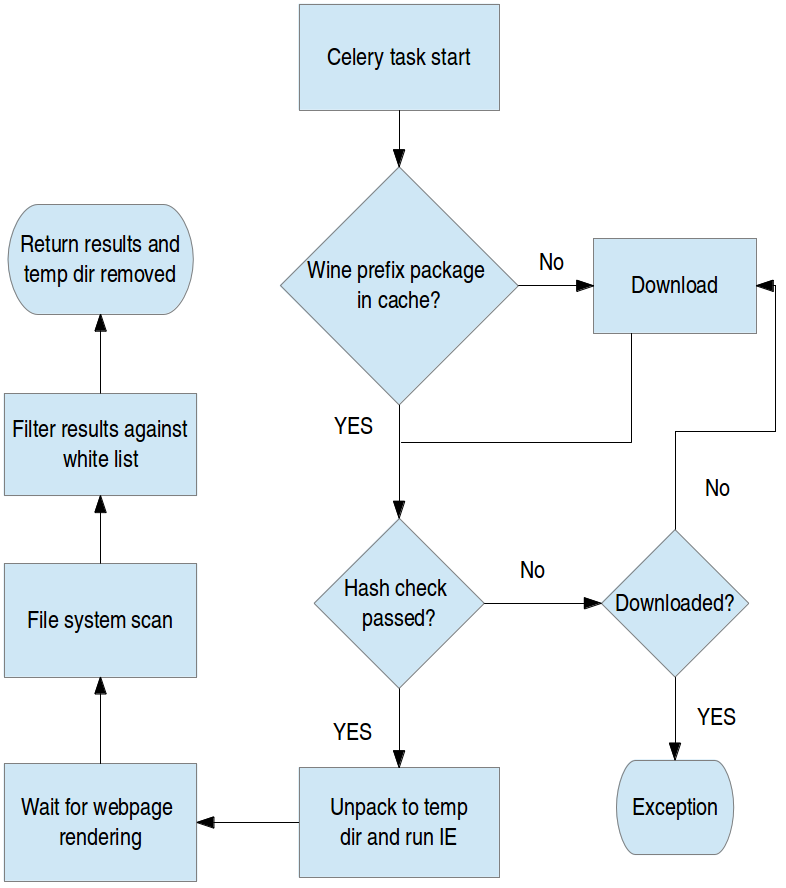
\includegraphics[width=0.8\textwidth]{img/wine-flowchart.png}
\caption{Program flow}
\label{fig:wine}
\end{figure}
With Wine Explorer, URLs given by the URL classifier are opened with the specific instance of Internet Explorer inside the Wine 
prefix. 
These URLs are said to be strongly suspicious of containing malware and are 
supposed to be investigated in depth. \\
In order to speed up Wine prefix creation, a clean Wine prefix packed with 
Internet Explorer 6 is prepared. Therefore whenever a new Wine prefix is needed, 
the only process is to unpack it to a desired location. 
The package's SHA-256 hash is calculated and stored in Wine Explorer so that 
its validity can be ensured. 
The package is then uploaded into a web drive and can be downloaded in 
order to increase the system's portability. \\
The system should also be able to store multiple instances of Wine prefixes 
and execute Internet Explorers in them concurrently. 
After an execution is completed a scan is performed to check file system 
modifications inside that Wine prefix. 
A white list is provided which describes files which might be modified by
system operations. 
The results are then returned to the main system, and the temporary Wine 
prefixes after scanning should be removed in order to save disk space. 

\subsection{Implementation}
Python is used to implement this program just as other parts of this project. 
WineBrowser, an instance of Wine prefix running it, manages all operations 
with a single URL. Details on how the program work are as follows:
\begin{enumerate}
\item \verb`create_wine_prefix(template_spec)` \\
Check cache for the package containing the predefined Wine prefix. If it does
not exist, download it, and perform a hash check.
If success the package is unpacked to a temporary directory. 
\item \verb`WineBrowser.__init__()` and \verb`WineBrowser.run()`\\
The active Wine prefix is set to the temporary directory, and the Internet 
Explorer is run with the given URL under Wine. 
\item
Wait for 30 seconds.
\item \verb`check_change(dir1,dir2)`\\
Check the file system changes. This is achieved by running {\em filecmp} recursively 
for all files between the clean Wine prefix and the active one. The results 
are filtered against a white list then returned to the main system. The white 
list is included in the appendix.%TODO 
\item \verb`WineBrowser.close()`\\
Remove the temporary directory. 
\end{enumerate}
Any web pages take more than 30 seconds to 
load will be discarded as one will significantly lower the system's 
throughput. \\
The main system runs one WineBrowser instance with Celery per task, in order 
to achieve concurrent execution of multiple Wine programs at the same time increases the overall throughput dramatically. 
